\documentclass[compress]{beamer}
\usetheme{metropolis}
\usepackage{tikz}
\usepackage{xcolor}
\usepackage[normalem]{ulem}

\definecolor{unipd}{RGB}{155, 0, 20}
\setbeamersize{text margin left=10pt, text margin right=10pt}

\title{New perspectives for developing short forms of tests}
\author{\begin{tabular}{rl}
		 Proponents:&  Ottavia M. Epifania, Rossella Caliciuri \\ 
		 Chair \& Discussant: & Rossella Caliciuri \\
	\end{tabular} }
\date{September 12, 2025}
\institute [] {
	\centering
	
\includegraphics[width=1.5cm,height=1.5cm,keepaspectratio]{img/unipd.png}%\hspace*{9.75cm}~%
	
\includegraphics[width=2.5cm,height=2.5cm,keepaspectratio]{img/psicostat.png}%
	
\includegraphics[width=1.5cm,height=1.5cm,keepaspectratio]{img/unicatt.png}%
	
\includegraphics[width=1.5cm,height=1.5cm,keepaspectratio]{img/FISPPA_logo}  \\
	
\includegraphics[width=1.5cm,height=1.5cm,keepaspectratio]{img/stat} 
	
\includegraphics[width=1.5cm,height=1.5cm,keepaspectratio]{img/unitn} 
		
\includegraphics[width=1.5cm,height=1.5cm,keepaspectratio]{img/dpg}
			
\includegraphics[width=1.5cm,height=1.5cm,keepaspectratio]{img/ITD}}
\begin{document}

\begin{frame}[plain]
    \maketitle
\end{frame}

\begin{frame}{Why?}
\pause

 \begin{tikzpicture}[remember picture, overlay]
	% Place the image
	\node[anchor=center] at (current page.center) {
		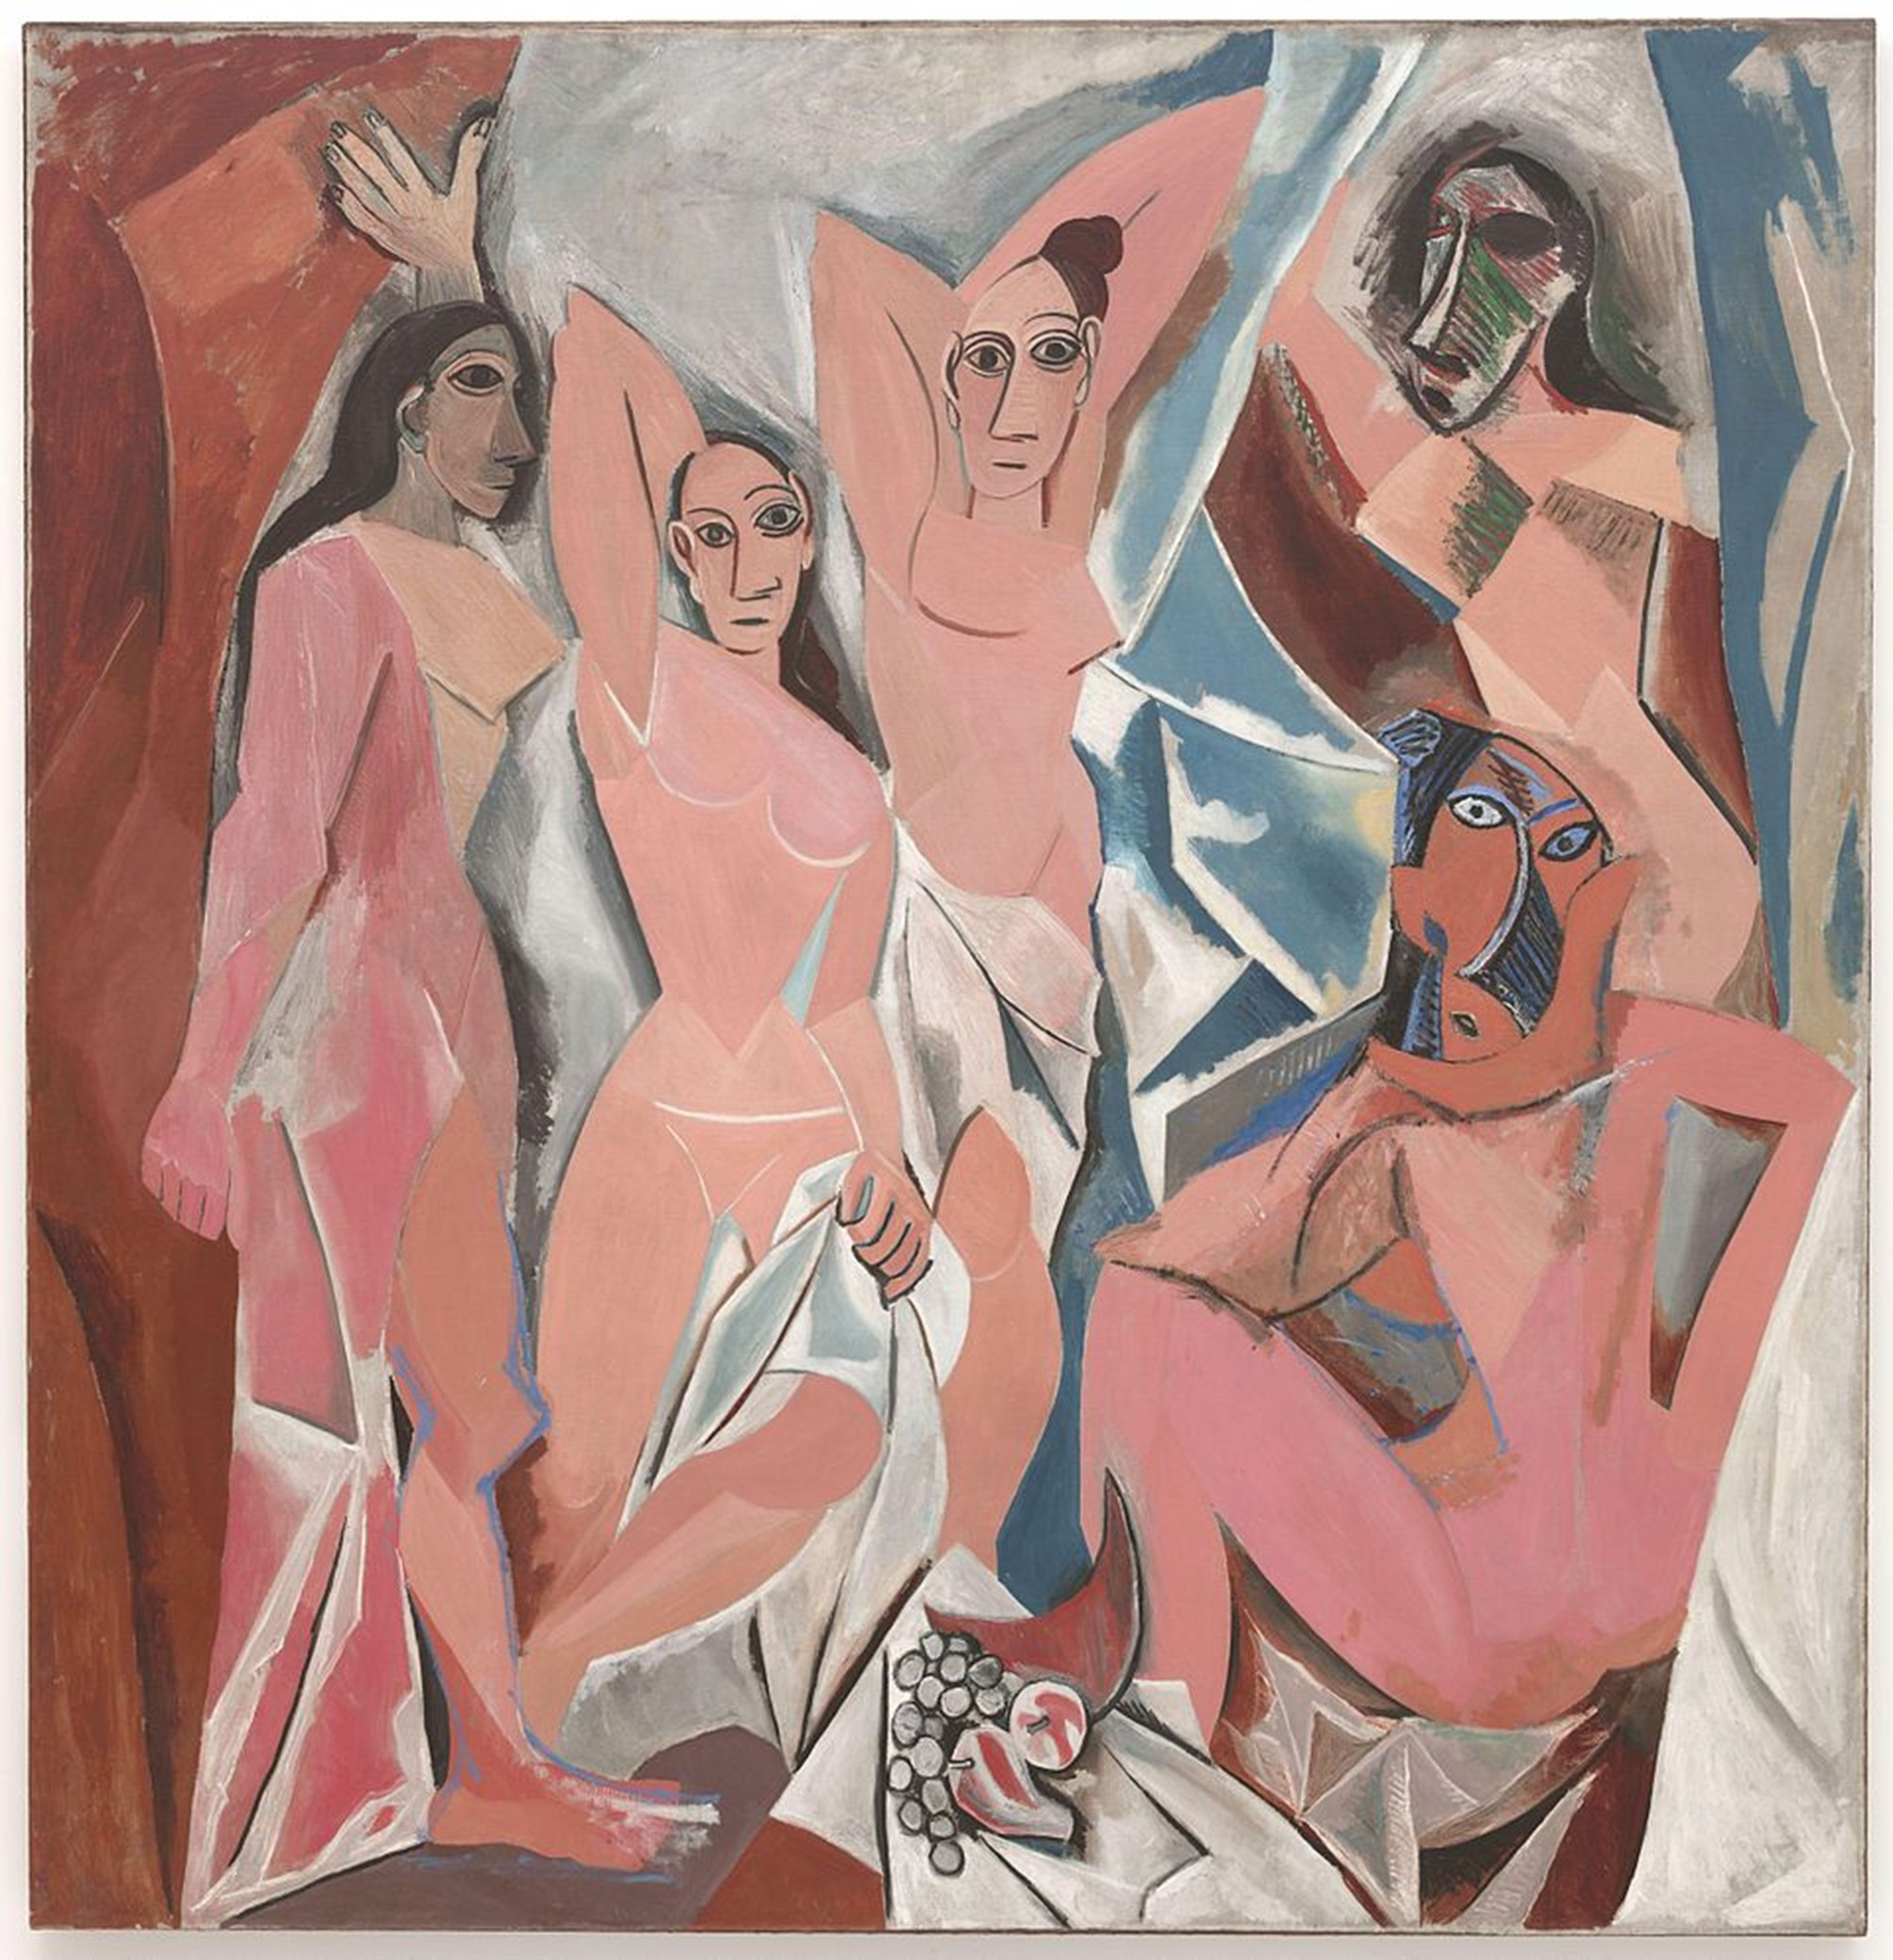
\includegraphics[width=0.8\textwidth]{img/dams} % Replace with your image file
	};
	
	
	\node[anchor=north west, xshift=-5cm,yshift=-0.5cm, fill=white!40, inner sep=2pt] at (current page.center) {
		\textcolor{unipd}{\Large \textbf{Competence-based Knowledge Space Theory}}
	};
	\node[anchor=north east, xshift=+3cm, yshift=+2cm, fill=white!40, inner sep=2pt] at (current page.center) {
		\textcolor{unipd}{\Large\textbf{Knowledge Space Theory}}
	};
	\node[anchor=north west, xshift=-3cm, fill=white!40,yshift=-2cm, inner sep=2pt] at (current page.center) {
		\textcolor{unipd}{\Large\textbf{Item Response Theory}}
	};
		\node[anchor=south east, xshift=3cm, fill=white!40, inner sep=2pt] at (current page.center) {
		\textcolor{unipd}{\Large\textbf{Machine Learning}}
	};
		\node[anchor=south, xshift=3cm, yshift=1cm, fill=white!40, inner sep=2pt] at (current page.south) {
		\textcolor{unipd}{\Large\textbf{Classical Test Theory}}
	};
\end{tikzpicture}



\end{frame}

\begin{frame}{Contributions}
	
	\small
	
\only<1>{
	\textbf{Measuring the Stability of Adaptive Psychological Assessment}
	
	{\footnotesize{Debora de Chiusole et al., \texttt{debora.dechiusole@unipd.it}}}
}

\only<2->{
	\textbf{\textcolor{unipd}{\sout{Measuring the Stability of Adaptive Psychological Assessment}}}
	
	{\footnotesize{\textcolor{unipd}{\sout{Debora de Chiusole et al., \texttt{debora.dechiusole@unipd.it}}}}}
}

	\onslide<3->
	

\textbf{More than a short form: Using adaptive assessments to optimize clinical insight from the first session}
	
	
{\footnotesize{Umberto	Granziol et al., \texttt{umberto.granziol@unipd.it}}} 
	
\onslide<4->
	
	\textbf{Shortening tests within competence-based knowledge space theory}
	

{\footnotesize{Pasquale Anselmi, \texttt{pasquale.anselmi@unipd.it}}}

\onslide<5->

	\textbf{Natural selection for items: Evaluating a genetic algorithm for developing questionnaire short forms}



{\footnotesize{Marcello Passarelli, \texttt{marcello.passarelli@cnr.it}}}

\onslide<6->

\textbf{Will the suffering ever end? An item response theory algorithm for shortening tests}

{\footnotesize{Ottavia Epifania et al., 
\includegraphics[width=.04\linewidth]{img/freepalestine} \texttt{ottavia.epifania@unitn.it}}} 


	
\end{frame}

\end{document}
